\onecolumn
\appendices
\renewcommand{\appendixname}{Annex}

\section{Data-Flow Diagram}
\label{ann:dfd}

Figure~\ref{fig:dfd} shows the level-1 \ac{DFD} used for threat
modelling. It refines the context diagram of Figure~\ref{fig:context}:
the backend is split into the \ac{API} gateway (P3), the identity and
access management service (P4) and the banking services (P5), and the
\ac{CI/CD} pipeline (P6) is added because it delivers the code that runs
in the data centre. EE3 is outside the product, as discussed in
Section~\ref{sec:cra}.

\begin{figure}[!h]
  \centering
  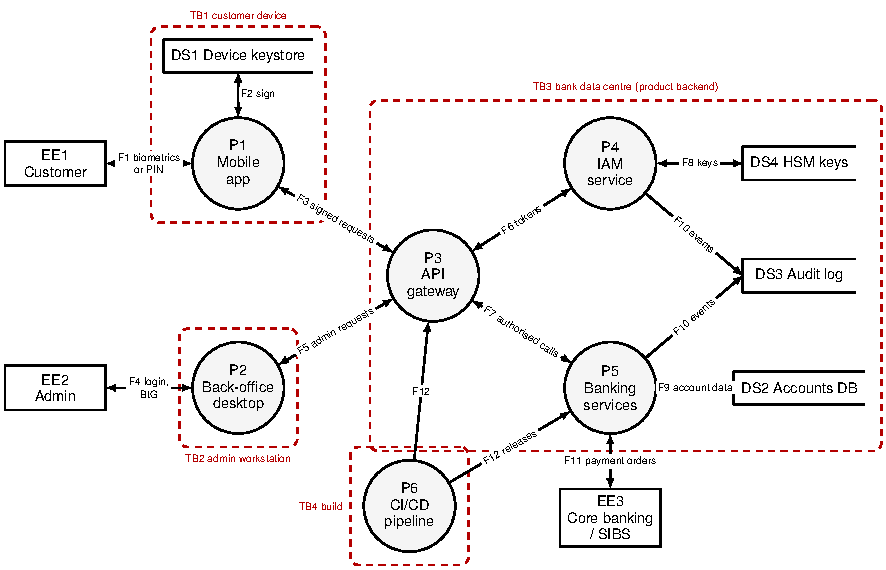
\includegraphics[width=0.75\textwidth]{DFD.pdf}
  \caption{Level-1 data-flow diagram of SecureBank PT with trust boundaries (TB1--TB4).}
  \label{fig:dfd}
\end{figure}

\section{Threat Table}
\label{ann:threats}

Table~\ref{tab:threats} lists the threats found by applying \ac{STRIDE} to
the elements of Figure~\ref{fig:dfd}, and the requirements of
Section~\ref{sec:catalogue} that answer each one.

\begin{table}[!h]
\caption{STRIDE threats on the data-flow diagram and the requirements that answer them}
\label{tab:threats}
\centering
\scriptsize
\begin{tabularx}{\textwidth}{@{}L{0.6cm}c@{\hspace{6pt}}L{1.3cm}YL{4.2cm}@{}}
\toprule
\textbf{ID} & \textbf{STRIDE} & \textbf{Element} & \textbf{Threat} & \textbf{Requirements} \\
\midrule
T01 & S & EE1, F1 & An attacker logs in with a \ac{PIN} obtained by phishing or by credential stuffing. & REQ-05, REQ-13, REQ-15, REQ-21 \\
T02 & S & F3 & A stolen access token is replayed from another device. & REQ-15, REQ-16 \\
T03 & S & P1 & A repackaged application or a fake bank website collects the \ac{PIN} and matrix codes and enrols an attacker device. & REQ-05, REQ-15 \\
T04 & S & DS1, P1 & A lost or stolen enrolled device is used by a third party. & REQ-15, REQ-19 \\
T05 & S & EE1, P1 & A fraudster impersonates a payee and leads the customer to pay a mule account. & REQ-20 \\
T06 & T & F3, P1 & The amount or payee is altered in transit or by malware on a rooted device. & REQ-06, REQ-22 \\
T07 & T & F3 & A captured signed transfer is replayed. & REQ-07 \\
T08 & T & P6, F12 & A malicious dependency or a tampered artefact is deployed. & REQ-10 \\
T09 & T & P5, F11 & A failure in the middle of a transfer leaves a partial debit. & REQ-08 \\
T10 & R & P5, DS3 & A customer or an Admin denies a transfer or an administrative action. & REQ-06, REQ-09 \\
T11 & R & DS3 & An insider edits or deletes audit records. & REQ-09, REQ-18 \\
T12 & I & F3 & A man-in-the-middle with a rogue certificate reads the client channel. & REQ-01, REQ-22 \\
T13 & I & DS1, P1 & Tokens or account data are read from a lost or rooted device. & REQ-03 \\
T14 & I & P3, P5 & A customer reads the data of another customer by changing an identifier in a request. & REQ-04, REQ-22 \\
T15 & I & DS2 & A copy of the database or of a backup is stolen. & REQ-02 \\
T16 & D & P3, F3 & A flood of requests targets the login and transfer endpoints. & REQ-11, REQ-12, REQ-21 \\
T17 & D & P4 & Customers are locked out by repeated wrong \acp{PIN}. & REQ-13, REQ-21 \\
T18 & D & P5, DS2 & A data centre failure or ransomware makes the backend data unavailable. & REQ-14 \\
T19 & E & P3, P4 & A customer token is used on back-office endpoints, or an Admin initiates a transfer. & REQ-17, REQ-22 \\
T20 & E & EE2, P2 & An Admin abuses privileged access to freeze accounts or read customer data. & REQ-09, REQ-18 \\
\bottomrule
\end{tabularx}
\end{table}
